\documentclass[1p]{elsarticle_modified}
%\bibliographystyle{elsarticle-num}

%\usepackage[colorlinks]{hyperref}
%\usepackage{abbrmath_seonhwa} %\Abb, \Ascr, \Acal ,\Abf, \Afrak
\usepackage{amsfonts}
\usepackage{amssymb}
\usepackage{amsmath}
\usepackage{amsthm}
\usepackage{scalefnt}
\usepackage{amsbsy}
\usepackage{kotex}
\usepackage{caption}
\usepackage{subfig}
\usepackage{color}
\usepackage{graphicx}
\usepackage{xcolor} %% white, black, red, green, blue, cyan, magenta, yellow
\usepackage{float}
\usepackage{setspace}
\usepackage{hyperref}

\usepackage{tikz}
\usetikzlibrary{arrows}

\usepackage{multirow}
\usepackage{array} % fixed length table
\usepackage{hhline}

%%%%%%%%%%%%%%%%%%%%%
\makeatletter
\renewcommand*\env@matrix[1][\arraystretch]{%
	\edef\arraystretch{#1}%
	\hskip -\arraycolsep
	\let\@ifnextchar\new@ifnextchar
	\array{*\c@MaxMatrixCols c}}
\makeatother %https://tex.stackexchange.com/questions/14071/how-can-i-increase-the-line-spacing-in-a-matrix
%%%%%%%%%%%%%%%

\usepackage[normalem]{ulem}

\newcommand{\msout}[1]{\ifmmode\text{\sout{\ensuremath{#1}}}\else\sout{#1}\fi}
%SOURCE: \msout is \stkout macro in https://tex.stackexchange.com/questions/20609/strikeout-in-math-mode

\newcommand{\cancel}[1]{
	\ifmmode
	{\color{red}\msout{#1}}
	\else
	{\color{red}\sout{#1}}
	\fi
}

\newcommand{\add}[1]{
	{\color{blue}\uwave{#1}}
}

\newcommand{\replace}[2]{
	\ifmmode
	{\color{red}\msout{#1}}{\color{blue}\uwave{#2}}
	\else
	{\color{red}\sout{#1}}{\color{blue}\uwave{#2}}
	\fi
}

\newcommand{\Sol}{\mathcal{S}} %segment
\newcommand{\D}{D} %diagram
\newcommand{\A}{\mathcal{A}} %arc


%%%%%%%%%%%%%%%%%%%%%%%%%%%%%5 test

\def\sl{\operatorname{\textup{SL}}(2,\Cbb)}
\def\psl{\operatorname{\textup{PSL}}(2,\Cbb)}
\def\quan{\mkern 1mu \triangleright \mkern 1mu}

\theoremstyle{definition}
\newtheorem{thm}{Theorem}[section]
\newtheorem{prop}[thm]{Proposition}
\newtheorem{lem}[thm]{Lemma}
\newtheorem{ques}[thm]{Question}
\newtheorem{cor}[thm]{Corollary}
\newtheorem{defn}[thm]{Definition}
\newtheorem{exam}[thm]{Example}
\newtheorem{rmk}[thm]{Remark}
\newtheorem{alg}[thm]{Algorithm}

\newcommand{\I}{\sqrt{-1}}
\begin{document}

%\begin{frontmatter}
%
%\title{Boundary parabolic representations of knots up to 8 crossings}
%
%%% Group authors per affiliation:
%\author{Yunhi Cho} 
%\address{Department of Mathematics, University of Seoul, Seoul, Korea}
%\ead{yhcho@uos.ac.kr}
%
%
%\author{Seonhwa Kim} %\fnref{s_kim}}
%\address{Center for Geometry and Physics, Institute for Basic Science, Pohang, 37673, Korea}
%\ead{ryeona17@ibs.re.kr}
%
%\author{Hyuk Kim}
%\address{Department of Mathematical Sciences, Seoul National University, Seoul 08826, Korea}
%\ead{hyukkim@snu.ac.kr}
%
%\author{Seokbeom Yoon}
%\address{Department of Mathematical Sciences, Seoul National University, Seoul, 08826,  Korea}
%\ead{sbyoon15@snu.ac.kr}
%
%\begin{abstract}
%We find all boundary parabolic representation of knots up to 8 crossings.
%
%\end{abstract}
%\begin{keyword}
%    \MSC[2010] 57M25 
%\end{keyword}
%
%\end{frontmatter}

%\linenumbers
%\tableofcontents
%
\newcommand\colored[1]{\textcolor{white}{\rule[-0.35ex]{0.8em}{1.4ex}}\kern-0.8em\color{red} #1}%
%\newcommand\colored[1]{\textcolor{white}{ #1}\kern-2.17ex	\textcolor{white}{ #1}\kern-1.81ex	\textcolor{white}{ #1}\kern-2.15ex\color{red}#1	}

{\Large $\underline{12a_{0385}~(K12a_{0385})}$}

\setlength{\tabcolsep}{10pt}
\renewcommand{\arraystretch}{1.6}
\vspace{1cm}\begin{tabular}{m{100pt}>{\centering\arraybackslash}m{274pt}}
\multirow{5}{120pt}{
	\centering
	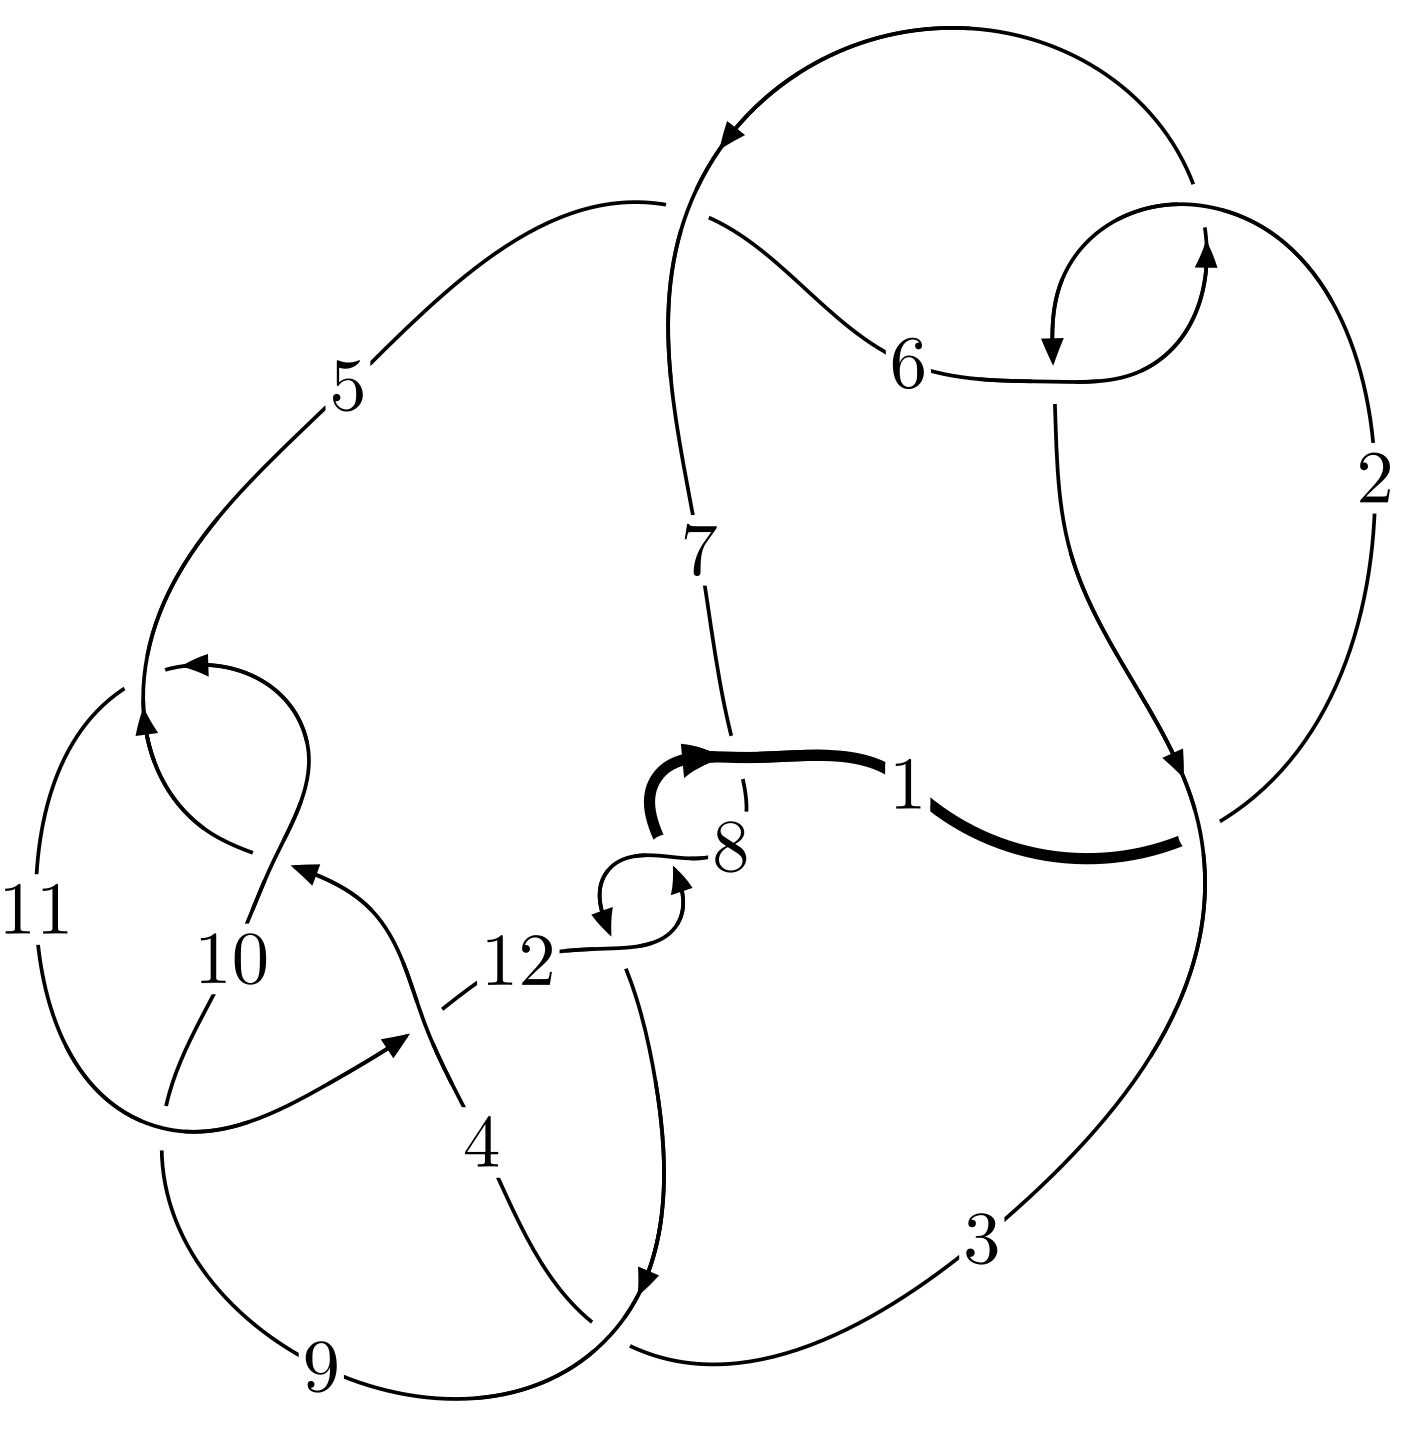
\includegraphics[width=112pt]{../../../GIT/diagram.site/Diagrams/png/1186_12a_0385.png}\\
\ \ \ A knot diagram\footnotemark}&
\allowdisplaybreaks
\textbf{Linearized knot diagam} \\
\cline{2-2}
 &
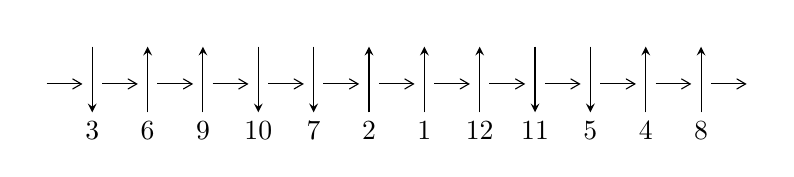
\begin{tikzpicture}[x=20pt, y=17pt]
	% nodes
	\node (C0) at (0, 0) {};
	\node (C1) at (1, 0) {};
	\node (C1U) at (1, +1) {};
	\node (C1D) at (1, -1) {3};

	\node (C2) at (2, 0) {};
	\node (C2U) at (2, +1) {};
	\node (C2D) at (2, -1) {6};

	\node (C3) at (3, 0) {};
	\node (C3U) at (3, +1) {};
	\node (C3D) at (3, -1) {9};

	\node (C4) at (4, 0) {};
	\node (C4U) at (4, +1) {};
	\node (C4D) at (4, -1) {10};

	\node (C5) at (5, 0) {};
	\node (C5U) at (5, +1) {};
	\node (C5D) at (5, -1) {7};

	\node (C6) at (6, 0) {};
	\node (C6U) at (6, +1) {};
	\node (C6D) at (6, -1) {2};

	\node (C7) at (7, 0) {};
	\node (C7U) at (7, +1) {};
	\node (C7D) at (7, -1) {1};

	\node (C8) at (8, 0) {};
	\node (C8U) at (8, +1) {};
	\node (C8D) at (8, -1) {12};

	\node (C9) at (9, 0) {};
	\node (C9U) at (9, +1) {};
	\node (C9D) at (9, -1) {11};

	\node (C10) at (10, 0) {};
	\node (C10U) at (10, +1) {};
	\node (C10D) at (10, -1) {5};

	\node (C11) at (11, 0) {};
	\node (C11U) at (11, +1) {};
	\node (C11D) at (11, -1) {4};

	\node (C12) at (12, 0) {};
	\node (C12U) at (12, +1) {};
	\node (C12D) at (12, -1) {8};
	\node (C13) at (13, 0) {};

	% arrows
	\draw[->,>={angle 60}]
	(C0) edge (C1) (C1) edge (C2) (C2) edge (C3) (C3) edge (C4) (C4) edge (C5) (C5) edge (C6) (C6) edge (C7) (C7) edge (C8) (C8) edge (C9) (C9) edge (C10) (C10) edge (C11) (C11) edge (C12) (C12) edge (C13) ;	\draw[->,>=stealth]
	(C1U) edge (C1D) (C2D) edge (C2U) (C3D) edge (C3U) (C4U) edge (C4D) (C5U) edge (C5D) (C6D) edge (C6U) (C7D) edge (C7U) (C8D) edge (C8U) (C9U) edge (C9D) (C10U) edge (C10D) (C11D) edge (C11U) (C12D) edge (C12U) ;
	\end{tikzpicture} \\
\hhline{~~} \\& 
\textbf{Solving Sequence} \\ \cline{2-2} 
 &
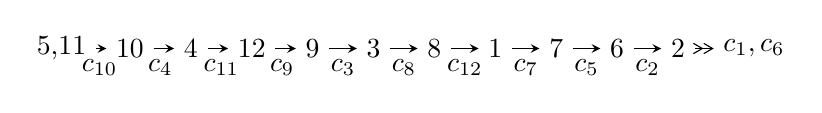
\begin{tikzpicture}[x=22pt, y=7pt]
	% node
	\node (A0) at (-1/8, 0) {5,11};
	\node (A1) at (1, 0) {10};
	\node (A2) at (2, 0) {4};
	\node (A3) at (3, 0) {12};
	\node (A4) at (4, 0) {9};
	\node (A5) at (5, 0) {3};
	\node (A6) at (6, 0) {8};
	\node (A7) at (7, 0) {1};
	\node (A8) at (8, 0) {7};
	\node (A9) at (9, 0) {6};
	\node (A10) at (10, 0) {2};
	\node (C1) at (1/2, -1) {$c_{10}$};
	\node (C2) at (3/2, -1) {$c_{4}$};
	\node (C3) at (5/2, -1) {$c_{11}$};
	\node (C4) at (7/2, -1) {$c_{9}$};
	\node (C5) at (9/2, -1) {$c_{3}$};
	\node (C6) at (11/2, -1) {$c_{8}$};
	\node (C7) at (13/2, -1) {$c_{12}$};
	\node (C8) at (15/2, -1) {$c_{7}$};
	\node (C9) at (17/2, -1) {$c_{5}$};
	\node (C10) at (19/2, -1) {$c_{2}$};
	\node (A11) at (45/4, 0) {$c_{1},c_{6}$};

	% edge
	\draw[->,>=stealth]	
	(A0) edge (A1) (A1) edge (A2) (A2) edge (A3) (A3) edge (A4) (A4) edge (A5) (A5) edge (A6) (A6) edge (A7) (A7) edge (A8) (A8) edge (A9) (A9) edge (A10) ;
	\draw[->>,>={angle 60}]	
	(A10) edge (A11);
\end{tikzpicture} \\ 

\end{tabular} \\

\footnotetext{
The image of knot diagram is generated by the software ``\textbf{Draw programme}" developed by Andrew Bartholomew(\url{http://www.layer8.co.uk/maths/draw/index.htm\#Running-draw}), where we modified some parts for our purpose(\url{https://github.com/CATsTAILs/LinksPainter}).
}\phantom \\ \newline 
\centering \textbf{Ideals for irreducible components\footnotemark of $X_{\text{par}}$} 
 
\begin{align*}
I^u_{1}&=\langle 
u^{80}+u^{79}+\cdots+2 u^4+1\rangle \\
\\
\end{align*}
\raggedright * 1 irreducible components of $\dim_{\mathbb{C}}=0$, with total 80 representations.\\
\footnotetext{All coefficients of polynomials are rational numbers. But the coefficients are sometimes approximated in decimal forms when there is not enough margin.}
\newpage
\renewcommand{\arraystretch}{1}
\centering \section*{I. $I^u_{1}= \langle u^{80}+u^{79}+\cdots+2 u^4+1 \rangle$}
\flushleft \textbf{(i) Arc colorings}\\
\begin{tabular}{m{7pt} m{180pt} m{7pt} m{180pt} }
\flushright $a_{5}=$&$\begin{pmatrix}0\\u\end{pmatrix}$ \\
\flushright $a_{11}=$&$\begin{pmatrix}1\\0\end{pmatrix}$ \\
\flushright $a_{10}=$&$\begin{pmatrix}1\\- u^2\end{pmatrix}$ \\
\flushright $a_{4}=$&$\begin{pmatrix}u\\- u^3+u\end{pmatrix}$ \\
\flushright $a_{12}=$&$\begin{pmatrix}u^4- u^2+1\\- u^6+2 u^4- u^2\end{pmatrix}$ \\
\flushright $a_{9}=$&$\begin{pmatrix}- u^2+1\\- u^2\end{pmatrix}$ \\
\flushright $a_{3}=$&$\begin{pmatrix}u^7-2 u^5+2 u^3\\u^7- u^5+u\end{pmatrix}$ \\
\flushright $a_{8}=$&$\begin{pmatrix}u^{12}-3 u^{10}+5 u^8-4 u^6+2 u^4- u^2+1\\- u^{14}+4 u^{12}-7 u^{10}+6 u^8-2 u^6- u^2\end{pmatrix}$ \\
\flushright $a_{1}=$&$\begin{pmatrix}u^{20}-5 u^{18}+13 u^{16}-20 u^{14}+20 u^{12}-13 u^{10}+7 u^8-4 u^6+3 u^4- u^2+1\\- u^{22}+6 u^{20}+\cdots+2 u^4- u^2\end{pmatrix}$ \\
\flushright $a_{7}=$&$\begin{pmatrix}u^{28}-7 u^{26}+\cdots- u^2+1\\- u^{30}+8 u^{28}+\cdots-4 u^6- u^2\end{pmatrix}$ \\
\flushright $a_{6}=$&$\begin{pmatrix}- u^{57}+14 u^{55}+\cdots+2 u^3- u\\u^{59}-15 u^{57}+\cdots+u^3+u\end{pmatrix}$ \\
\flushright $a_{2}=$&$\begin{pmatrix}u^{36}-9 u^{34}+\cdots- u^2+1\\u^{36}-8 u^{34}+\cdots-4 u^8+u^4\end{pmatrix}$\\&\end{tabular}
\flushleft \textbf{(ii) Obstruction class $= -1$}\\~\\
\flushleft \textbf{(iii) Cusp Shapes $= 4 u^{78}-76 u^{76}+\cdots-4 u+2$}\\~\\
\newpage\renewcommand{\arraystretch}{1}
\flushleft \textbf{(iv) u-Polynomials at the component}\newline \\
\begin{tabular}{m{50pt}|m{274pt}}
Crossings & \hspace{64pt}u-Polynomials at each crossing \\
\hline $$\begin{aligned}c_{1},c_{5}\end{aligned}$$&$\begin{aligned}
&u^{80}+29 u^{79}+\cdots-8 u^2+1
\end{aligned}$\\
\hline $$\begin{aligned}c_{2},c_{6}\end{aligned}$$&$\begin{aligned}
&u^{80}- u^{79}+\cdots-4 u^3+1
\end{aligned}$\\
\hline $$\begin{aligned}c_{3}\end{aligned}$$&$\begin{aligned}
&u^{80}+u^{79}+\cdots+256 u+97
\end{aligned}$\\
\hline $$\begin{aligned}c_{4},c_{10}\end{aligned}$$&$\begin{aligned}
&u^{80}- u^{79}+\cdots+2 u^4+1
\end{aligned}$\\
\hline $$\begin{aligned}c_{7},c_{8},c_{12}\end{aligned}$$&$\begin{aligned}
&u^{80}+5 u^{79}+\cdots+24 u+1
\end{aligned}$\\
\hline $$\begin{aligned}c_{9}\end{aligned}$$&$\begin{aligned}
&u^{80}+39 u^{79}+\cdots+4 u^2+1
\end{aligned}$\\
\hline $$\begin{aligned}c_{11}\end{aligned}$$&$\begin{aligned}
&u^{80}-3 u^{79}+\cdots+800 u+851
\end{aligned}$\\
\hline
\end{tabular}\\~\\
\newpage\renewcommand{\arraystretch}{1}
\flushleft \textbf{(v) Riley Polynomials at the component}\newline \\
\begin{tabular}{m{50pt}|m{274pt}}
Crossings & \hspace{64pt}Riley Polynomials at each crossing \\
\hline $$\begin{aligned}c_{1},c_{5}\end{aligned}$$&$\begin{aligned}
&y^{80}+45 y^{79}+\cdots-16 y+1
\end{aligned}$\\
\hline $$\begin{aligned}c_{2},c_{6}\end{aligned}$$&$\begin{aligned}
&y^{80}+29 y^{79}+\cdots-8 y^2+1
\end{aligned}$\\
\hline $$\begin{aligned}c_{3}\end{aligned}$$&$\begin{aligned}
&y^{80}+9 y^{79}+\cdots+10512 y+9409
\end{aligned}$\\
\hline $$\begin{aligned}c_{4},c_{10}\end{aligned}$$&$\begin{aligned}
&y^{80}-39 y^{79}+\cdots+4 y^2+1
\end{aligned}$\\
\hline $$\begin{aligned}c_{7},c_{8},c_{12}\end{aligned}$$&$\begin{aligned}
&y^{80}+81 y^{79}+\cdots+8 y+1
\end{aligned}$\\
\hline $$\begin{aligned}c_{9}\end{aligned}$$&$\begin{aligned}
&y^{80}+5 y^{79}+\cdots+8 y+1
\end{aligned}$\\
\hline $$\begin{aligned}c_{11}\end{aligned}$$&$\begin{aligned}
&y^{80}+29 y^{79}+\cdots+19021504 y+724201
\end{aligned}$\\
\hline
\end{tabular}\\~\\
\newpage\flushleft \textbf{(vi) Complex Volumes and Cusp Shapes}
$$\begin{array}{c|c|c}  
\text{Solutions to }I^u_{1}& \I (\text{vol} + \sqrt{-1}CS) & \text{Cusp shape}\\
 \hline 
\begin{aligned}
u &= \phantom{-}0.974248 + 0.243707 I\end{aligned}
 & -0.341105 - 0.923106 I & \phantom{-0.000000 } 0 \\ \hline\begin{aligned}
u &= \phantom{-}0.974248 - 0.243707 I\end{aligned}
 & -0.341105 + 0.923106 I & \phantom{-0.000000 } 0 \\ \hline\begin{aligned}
u &= -0.798815 + 0.582962 I\end{aligned}
 & -2.45122 - 4.26356 I & \phantom{-0.000000 } 0 \\ \hline\begin{aligned}
u &= -0.798815 - 0.582962 I\end{aligned}
 & -2.45122 + 4.26356 I & \phantom{-0.000000 } 0 \\ \hline\begin{aligned}
u &= -0.760408 + 0.601524 I\end{aligned}
 & -6.49087 + 2.34742 I & -2.84735 - 3.42112 I \\ \hline\begin{aligned}
u &= -0.760408 - 0.601524 I\end{aligned}
 & -6.49087 - 2.34742 I & -2.84735 + 3.42112 I \\ \hline\begin{aligned}
u &= \phantom{-}0.784181 + 0.559828 I\end{aligned}
 & -1.03117 - 1.02296 I & \phantom{-}3.10972 + 3.14213 I \\ \hline\begin{aligned}
u &= \phantom{-}0.784181 - 0.559828 I\end{aligned}
 & -1.03117 + 1.02296 I & \phantom{-}3.10972 - 3.14213 I \\ \hline\begin{aligned}
u &= -0.728858 + 0.618278 I\end{aligned}
 & -2.22839 + 8.96435 I & \phantom{-}2.00000 - 8.27939 I \\ \hline\begin{aligned}
u &= -0.728858 - 0.618278 I\end{aligned}
 & -2.22839 - 8.96435 I & \phantom{-}2.00000 + 8.27939 I \\ \hline\begin{aligned}
u &= -1.029920 + 0.233477 I\end{aligned}
 & -1.08076 - 4.22509 I & \phantom{-0.000000 } 0 \\ \hline\begin{aligned}
u &= -1.029920 - 0.233477 I\end{aligned}
 & -1.08076 + 4.22509 I & \phantom{-0.000000 } 0 \\ \hline\begin{aligned}
u &= \phantom{-}0.723078 + 0.602518 I\end{aligned}
 & -0.81811 - 3.55737 I & \phantom{-}3.81185 + 3.70716 I \\ \hline\begin{aligned}
u &= \phantom{-}0.723078 - 0.602518 I\end{aligned}
 & -0.81811 + 3.55737 I & \phantom{-}3.81185 - 3.70716 I \\ \hline\begin{aligned}
u &= \phantom{-}1.021260 + 0.405865 I\end{aligned}
 & -1.70172 - 1.76133 I & \phantom{-0.000000 } 0 \\ \hline\begin{aligned}
u &= \phantom{-}1.021260 - 0.405865 I\end{aligned}
 & -1.70172 + 1.76133 I & \phantom{-0.000000 } 0 \\ \hline\begin{aligned}
u &= -1.075770 + 0.327642 I\end{aligned}
 & -5.25765 + 0.50983 I & \phantom{-0.000000 } 0 \\ \hline\begin{aligned}
u &= -1.075770 - 0.327642 I\end{aligned}
 & -5.25765 - 0.50983 I & \phantom{-0.000000 } 0 \\ \hline\begin{aligned}
u &= \phantom{-}0.996305 + 0.530127 I\end{aligned}
 & \phantom{-}2.55643 + 0.13963 I & \phantom{-0.000000 } 0 \\ \hline\begin{aligned}
u &= \phantom{-}0.996305 - 0.530127 I\end{aligned}
 & \phantom{-}2.55643 - 0.13963 I & \phantom{-0.000000 } 0 \\ \hline\begin{aligned}
u &= -1.014540 + 0.534615 I\end{aligned}
 & \phantom{-}2.77964 + 5.23374 I & \phantom{-0.000000 } 0 \\ \hline\begin{aligned}
u &= -1.014540 - 0.534615 I\end{aligned}
 & \phantom{-}2.77964 - 5.23374 I & \phantom{-0.000000 } 0 \\ \hline\begin{aligned}
u &= -1.094730 + 0.408125 I\end{aligned}
 & -2.84165 + 5.68344 I & \phantom{-0.000000 } 0 \\ \hline\begin{aligned}
u &= -1.094730 - 0.408125 I\end{aligned}
 & -2.84165 - 5.68344 I & \phantom{-0.000000 } 0 \\ \hline\begin{aligned}
u &= -0.276879 + 0.781910 I\end{aligned}
 & -4.43959 - 10.77180 I & \phantom{-}0.62357 + 6.97709 I \\ \hline\begin{aligned}
u &= -0.276879 - 0.781910 I\end{aligned}
 & -4.43959 + 10.77180 I & \phantom{-}0.62357 - 6.97709 I \\ \hline\begin{aligned}
u &= \phantom{-}0.275922 + 0.773655 I\end{aligned}
 & -2.95631 + 5.26247 I & \phantom{-}2.70471 - 2.47758 I \\ \hline\begin{aligned}
u &= \phantom{-}0.275922 - 0.773655 I\end{aligned}
 & -2.95631 - 5.26247 I & \phantom{-}2.70471 + 2.47758 I \\ \hline\begin{aligned}
u &= -0.258532 + 0.778086 I\end{aligned}
 & -8.88148 - 3.93678 I & -3.71532 + 2.43295 I \\ \hline\begin{aligned}
u &= -0.258532 - 0.778086 I\end{aligned}
 & -8.88148 + 3.93678 I & -3.71532 - 2.43295 I\\
 \hline 
 \end{array}$$\newpage$$\begin{array}{c|c|c}  
\text{Solutions to }I^u_{1}& \I (\text{vol} + \sqrt{-1}CS) & \text{Cusp shape}\\
 \hline 
\begin{aligned}
u &= \phantom{-}0.549018 + 0.608925 I\end{aligned}
 & \phantom{-}3.86584 - 4.65764 I & \phantom{-}7.60494 + 6.72667 I \\ \hline\begin{aligned}
u &= \phantom{-}0.549018 - 0.608925 I\end{aligned}
 & \phantom{-}3.86584 + 4.65764 I & \phantom{-}7.60494 - 6.72667 I \\ \hline\begin{aligned}
u &= -1.071790 + 0.510904 I\end{aligned}
 & -0.83622 + 4.86099 I & \phantom{-0.000000 } 0 \\ \hline\begin{aligned}
u &= -1.071790 - 0.510904 I\end{aligned}
 & -0.83622 - 4.86099 I & \phantom{-0.000000 } 0 \\ \hline\begin{aligned}
u &= \phantom{-}1.094840 + 0.465113 I\end{aligned}
 & -2.46387 - 1.65619 I & \phantom{-0.000000 } 0 \\ \hline\begin{aligned}
u &= \phantom{-}1.094840 - 0.465113 I\end{aligned}
 & -2.46387 + 1.65619 I & \phantom{-0.000000 } 0 \\ \hline\begin{aligned}
u &= -0.238763 + 0.767511 I\end{aligned}
 & -4.99864 + 2.98355 I & -0.37409 - 2.63773 I \\ \hline\begin{aligned}
u &= -0.238763 - 0.767511 I\end{aligned}
 & -4.99864 - 2.98355 I & -0.37409 + 2.63773 I \\ \hline\begin{aligned}
u &= -0.519171 + 0.612965 I\end{aligned}
 & \phantom{-}4.23043 - 0.69017 I & \phantom{-}8.91098 - 0.24136 I \\ \hline\begin{aligned}
u &= -0.519171 - 0.612965 I\end{aligned}
 & \phantom{-}4.23043 + 0.69017 I & \phantom{-}8.91098 + 0.24136 I \\ \hline\begin{aligned}
u &= -1.164900 + 0.276437 I\end{aligned}
 & -7.38303 - 2.10122 I & \phantom{-0.000000 } 0 \\ \hline\begin{aligned}
u &= -1.164900 - 0.276437 I\end{aligned}
 & -7.38303 + 2.10122 I & \phantom{-0.000000 } 0 \\ \hline\begin{aligned}
u &= \phantom{-}0.249372 + 0.759552 I\end{aligned}
 & -3.37040 + 2.27685 I & \phantom{-}2.08581 - 2.28652 I \\ \hline\begin{aligned}
u &= \phantom{-}0.249372 - 0.759552 I\end{aligned}
 & -3.37040 - 2.27685 I & \phantom{-}2.08581 + 2.28652 I \\ \hline\begin{aligned}
u &= -1.164180 + 0.297688 I\end{aligned}
 & -7.64026 + 0.98754 I & \phantom{-0.000000 } 0 \\ \hline\begin{aligned}
u &= -1.164180 - 0.297688 I\end{aligned}
 & -7.64026 - 0.98754 I & \phantom{-0.000000 } 0 \\ \hline\begin{aligned}
u &= \phantom{-}1.170650 + 0.272859 I\end{aligned}
 & -8.91819 + 7.58864 I & \phantom{-0.000000 } 0 \\ \hline\begin{aligned}
u &= \phantom{-}1.170650 - 0.272859 I\end{aligned}
 & -8.91819 - 7.58864 I & \phantom{-0.000000 } 0 \\ \hline\begin{aligned}
u &= \phantom{-}1.173220 + 0.286979 I\end{aligned}
 & -13.27670 + 0.66412 I & \phantom{-0.000000 } 0 \\ \hline\begin{aligned}
u &= \phantom{-}1.173220 - 0.286979 I\end{aligned}
 & -13.27670 - 0.66412 I & \phantom{-0.000000 } 0 \\ \hline\begin{aligned}
u &= \phantom{-}1.171100 + 0.302065 I\end{aligned}
 & -9.27591 - 6.32389 I & \phantom{-0.000000 } 0 \\ \hline\begin{aligned}
u &= \phantom{-}1.171100 - 0.302065 I\end{aligned}
 & -9.27591 + 6.32389 I & \phantom{-0.000000 } 0 \\ \hline\begin{aligned}
u &= \phantom{-}0.367617 + 0.693910 I\end{aligned}
 & \phantom{-}3.06846 + 6.42905 I & \phantom{-}5.74931 - 6.97675 I \\ \hline\begin{aligned}
u &= \phantom{-}0.367617 - 0.693910 I\end{aligned}
 & \phantom{-}3.06846 - 6.42905 I & \phantom{-}5.74931 + 6.97675 I \\ \hline\begin{aligned}
u &= -1.085380 + 0.549352 I\end{aligned}
 & \phantom{-}1.61197 + 5.79661 I & \phantom{-0.000000 } 0 \\ \hline\begin{aligned}
u &= -1.085380 - 0.549352 I\end{aligned}
 & \phantom{-}1.61197 - 5.79661 I & \phantom{-0.000000 } 0 \\ \hline\begin{aligned}
u &= -0.383920 + 0.675789 I\end{aligned}
 & \phantom{-}3.65049 - 1.05201 I & \phantom{-}7.59735 + 1.19575 I \\ \hline\begin{aligned}
u &= -0.383920 - 0.675789 I\end{aligned}
 & \phantom{-}3.65049 + 1.05201 I & \phantom{-}7.59735 - 1.19575 I \\ \hline\begin{aligned}
u &= \phantom{-}1.107480 + 0.519195 I\end{aligned}
 & -3.96203 - 6.81758 I & \phantom{-0.000000 } 0 \\ \hline\begin{aligned}
u &= \phantom{-}1.107480 - 0.519195 I\end{aligned}
 & -3.96203 + 6.81758 I & \phantom{-0.000000 } 0\\
 \hline 
 \end{array}$$\newpage$$\begin{array}{c|c|c}  
\text{Solutions to }I^u_{1}& \I (\text{vol} + \sqrt{-1}CS) & \text{Cusp shape}\\
 \hline 
\begin{aligned}
u &= \phantom{-}1.094630 + 0.552876 I\end{aligned}
 & \phantom{-}0.95490 - 11.22700 I & \phantom{-0.000000 } 0 \\ \hline\begin{aligned}
u &= \phantom{-}1.094630 - 0.552876 I\end{aligned}
 & \phantom{-}0.95490 + 11.22700 I & \phantom{-0.000000 } 0 \\ \hline\begin{aligned}
u &= \phantom{-}0.616209 + 0.411830 I\end{aligned}
 & -0.52415 - 1.55757 I & -0.03671 + 5.81499 I \\ \hline\begin{aligned}
u &= \phantom{-}0.616209 - 0.411830 I\end{aligned}
 & -0.52415 + 1.55757 I & -0.03671 - 5.81499 I \\ \hline\begin{aligned}
u &= \phantom{-}1.147140 + 0.540994 I\end{aligned}
 & -5.98702 - 7.15179 I & \phantom{-0.000000 } 0 \\ \hline\begin{aligned}
u &= \phantom{-}1.147140 - 0.540994 I\end{aligned}
 & -5.98702 + 7.15179 I & \phantom{-0.000000 } 0 \\ \hline\begin{aligned}
u &= -1.152090 + 0.538667 I\end{aligned}
 & -7.66641 + 1.89692 I & \phantom{-0.000000 } 0 \\ \hline\begin{aligned}
u &= -1.152090 - 0.538667 I\end{aligned}
 & -7.66641 - 1.89692 I & \phantom{-0.000000 } 0 \\ \hline\begin{aligned}
u &= \phantom{-}1.146000 + 0.553071 I\end{aligned}
 & -5.50832 - 10.23230 I & \phantom{-0.000000 } 0 \\ \hline\begin{aligned}
u &= \phantom{-}1.146000 - 0.553071 I\end{aligned}
 & -5.50832 + 10.23230 I & \phantom{-0.000000 } 0 \\ \hline\begin{aligned}
u &= -1.151650 + 0.548129 I\end{aligned}
 & -11.5016 + 8.8913 I & \phantom{-0.000000 } 0 \\ \hline\begin{aligned}
u &= -1.151650 - 0.548129 I\end{aligned}
 & -11.5016 - 8.8913 I & \phantom{-0.000000 } 0 \\ \hline\begin{aligned}
u &= -1.148500 + 0.555482 I\end{aligned}
 & -7.0021 + 15.7722 I & \phantom{-0.000000 } 0 \\ \hline\begin{aligned}
u &= -1.148500 - 0.555482 I\end{aligned}
 & -7.0021 - 15.7722 I & \phantom{-0.000000 } 0 \\ \hline\begin{aligned}
u &= \phantom{-}0.275856 + 0.642568 I\end{aligned}
 & -1.60956 + 2.29309 I & -2.09430 - 4.60338 I \\ \hline\begin{aligned}
u &= \phantom{-}0.275856 - 0.642568 I\end{aligned}
 & -1.60956 - 2.29309 I & -2.09430 + 4.60338 I \\ \hline\begin{aligned}
u &= -0.387189 + 0.554390 I\end{aligned}
 & \phantom{-}1.139690 - 0.526971 I & \phantom{-}8.40078 + 1.81328 I \\ \hline\begin{aligned}
u &= -0.387189 - 0.554390 I\end{aligned}
 & \phantom{-}1.139690 + 0.526971 I & \phantom{-}8.40078 - 1.81328 I \\ \hline\begin{aligned}
u &= \phantom{-}0.067865 + 0.548015 I\end{aligned}
 & \phantom{-}0.15131 - 2.22893 I & \phantom{-}0.09814 + 3.20079 I \\ \hline\begin{aligned}
u &= \phantom{-}0.067865 - 0.548015 I\end{aligned}
 & \phantom{-}0.15131 + 2.22893 I & \phantom{-}0.09814 - 3.20079 I\\
 \hline 
 \end{array}$$\newpage
\newpage\renewcommand{\arraystretch}{1}
\centering \section*{ II. u-Polynomials}
\begin{tabular}{m{50pt}|m{274pt}}
Crossings & \hspace{64pt}u-Polynomials at each crossing \\
\hline $$\begin{aligned}c_{1},c_{5}\end{aligned}$$&$\begin{aligned}
&u^{80}+29 u^{79}+\cdots-8 u^2+1
\end{aligned}$\\
\hline $$\begin{aligned}c_{2},c_{6}\end{aligned}$$&$\begin{aligned}
&u^{80}- u^{79}+\cdots-4 u^3+1
\end{aligned}$\\
\hline $$\begin{aligned}c_{3}\end{aligned}$$&$\begin{aligned}
&u^{80}+u^{79}+\cdots+256 u+97
\end{aligned}$\\
\hline $$\begin{aligned}c_{4},c_{10}\end{aligned}$$&$\begin{aligned}
&u^{80}- u^{79}+\cdots+2 u^4+1
\end{aligned}$\\
\hline $$\begin{aligned}c_{7},c_{8},c_{12}\end{aligned}$$&$\begin{aligned}
&u^{80}+5 u^{79}+\cdots+24 u+1
\end{aligned}$\\
\hline $$\begin{aligned}c_{9}\end{aligned}$$&$\begin{aligned}
&u^{80}+39 u^{79}+\cdots+4 u^2+1
\end{aligned}$\\
\hline $$\begin{aligned}c_{11}\end{aligned}$$&$\begin{aligned}
&u^{80}-3 u^{79}+\cdots+800 u+851
\end{aligned}$\\
\hline
\end{tabular}\newpage\renewcommand{\arraystretch}{1}
\centering \section*{ III. Riley Polynomials}
\begin{tabular}{m{50pt}|m{274pt}}
Crossings & \hspace{64pt}Riley Polynomials at each crossing \\
\hline $$\begin{aligned}c_{1},c_{5}\end{aligned}$$&$\begin{aligned}
&y^{80}+45 y^{79}+\cdots-16 y+1
\end{aligned}$\\
\hline $$\begin{aligned}c_{2},c_{6}\end{aligned}$$&$\begin{aligned}
&y^{80}+29 y^{79}+\cdots-8 y^2+1
\end{aligned}$\\
\hline $$\begin{aligned}c_{3}\end{aligned}$$&$\begin{aligned}
&y^{80}+9 y^{79}+\cdots+10512 y+9409
\end{aligned}$\\
\hline $$\begin{aligned}c_{4},c_{10}\end{aligned}$$&$\begin{aligned}
&y^{80}-39 y^{79}+\cdots+4 y^2+1
\end{aligned}$\\
\hline $$\begin{aligned}c_{7},c_{8},c_{12}\end{aligned}$$&$\begin{aligned}
&y^{80}+81 y^{79}+\cdots+8 y+1
\end{aligned}$\\
\hline $$\begin{aligned}c_{9}\end{aligned}$$&$\begin{aligned}
&y^{80}+5 y^{79}+\cdots+8 y+1
\end{aligned}$\\
\hline $$\begin{aligned}c_{11}\end{aligned}$$&$\begin{aligned}
&y^{80}+29 y^{79}+\cdots+19021504 y+724201
\end{aligned}$\\
\hline
\end{tabular}
\vskip 2pc
\end{document}